% GNUPLOT: LaTeX picture with Postscript
\begingroup
  \makeatletter
  \providecommand\color[2][]{%
    \GenericError{(gnuplot) \space\space\space\@spaces}{%
      Package color not loaded in conjunction with
      terminal option `colourtext'%
    }{See the gnuplot documentation for explanation.%
    }{Either use 'blacktext' in gnuplot or load the package
      color.sty in LaTeX.}%
    \renewcommand\color[2][]{}%
  }%
  \providecommand\includegraphics[2][]{%
    \GenericError{(gnuplot) \space\space\space\@spaces}{%
      Package graphicx or graphics not loaded%
    }{See the gnuplot documentation for explanation.%
    }{The gnuplot epslatex terminal needs graphicx.sty or graphics.sty.}%
    \renewcommand\includegraphics[2][]{}%
  }%
  \providecommand\rotatebox[2]{#2}%
  \@ifundefined{ifGPcolor}{%
    \newif\ifGPcolor
    \GPcolortrue
  }{}%
  \@ifundefined{ifGPblacktext}{%
    \newif\ifGPblacktext
    \GPblacktexttrue
  }{}%
  % define a \g@addto@macro without @ in the name:
  \let\gplgaddtomacro\g@addto@macro
  % define empty templates for all commands taking text:
  \gdef\gplbacktext{}%
  \gdef\gplfronttext{}%
  \makeatother
  \ifGPblacktext
    % no textcolor at all
    \def\colorrgb#1{}%
    \def\colorgray#1{}%
  \else
    % gray or color?
    \ifGPcolor
      \def\colorrgb#1{\color[rgb]{#1}}%
      \def\colorgray#1{\color[gray]{#1}}%
      \expandafter\def\csname LTw\endcsname{\color{white}}%
      \expandafter\def\csname LTb\endcsname{\color{black}}%
      \expandafter\def\csname LTa\endcsname{\color{black}}%
      \expandafter\def\csname LT0\endcsname{\color[rgb]{1,0,0}}%
      \expandafter\def\csname LT1\endcsname{\color[rgb]{0,1,0}}%
      \expandafter\def\csname LT2\endcsname{\color[rgb]{0,0,1}}%
      \expandafter\def\csname LT3\endcsname{\color[rgb]{1,0,1}}%
      \expandafter\def\csname LT4\endcsname{\color[rgb]{0,1,1}}%
      \expandafter\def\csname LT5\endcsname{\color[rgb]{1,1,0}}%
      \expandafter\def\csname LT6\endcsname{\color[rgb]{0,0,0}}%
      \expandafter\def\csname LT7\endcsname{\color[rgb]{1,0.3,0}}%
      \expandafter\def\csname LT8\endcsname{\color[rgb]{0.5,0.5,0.5}}%
    \else
      % gray
      \def\colorrgb#1{\color{black}}%
      \def\colorgray#1{\color[gray]{#1}}%
      \expandafter\def\csname LTw\endcsname{\color{white}}%
      \expandafter\def\csname LTb\endcsname{\color{black}}%
      \expandafter\def\csname LTa\endcsname{\color{black}}%
      \expandafter\def\csname LT0\endcsname{\color{black}}%
      \expandafter\def\csname LT1\endcsname{\color{black}}%
      \expandafter\def\csname LT2\endcsname{\color{black}}%
      \expandafter\def\csname LT3\endcsname{\color{black}}%
      \expandafter\def\csname LT4\endcsname{\color{black}}%
      \expandafter\def\csname LT5\endcsname{\color{black}}%
      \expandafter\def\csname LT6\endcsname{\color{black}}%
      \expandafter\def\csname LT7\endcsname{\color{black}}%
      \expandafter\def\csname LT8\endcsname{\color{black}}%
    \fi
  \fi
    \setlength{\unitlength}{0.0500bp}%
    \ifx\gptboxheight\undefined%
      \newlength{\gptboxheight}%
      \newlength{\gptboxwidth}%
      \newsavebox{\gptboxtext}%
    \fi%
    \setlength{\fboxrule}{0.5pt}%
    \setlength{\fboxsep}{1pt}%
    \definecolor{tbcol}{rgb}{1,1,1}%
\begin{picture}(8500.00,6220.00)%
    \gplgaddtomacro\gplbacktext{%
      \csname LTb\endcsname%%
      \put(438,3416){\makebox(0,0)[r]{\strut{}$-8$}}%
      \csname LTb\endcsname%%
      \put(438,3705){\makebox(0,0)[r]{\strut{}$-6$}}%
      \csname LTb\endcsname%%
      \put(438,3993){\makebox(0,0)[r]{\strut{}$-4$}}%
      \csname LTb\endcsname%%
      \put(438,4282){\makebox(0,0)[r]{\strut{}$-2$}}%
      \csname LTb\endcsname%%
      \put(438,4570){\makebox(0,0)[r]{\strut{}$0$}}%
      \csname LTb\endcsname%%
      \put(438,4859){\makebox(0,0)[r]{\strut{}$2$}}%
      \csname LTb\endcsname%%
      \put(438,5147){\makebox(0,0)[r]{\strut{}$4$}}%
      \csname LTb\endcsname%%
      \put(438,5436){\makebox(0,0)[r]{\strut{}$6$}}%
      \csname LTb\endcsname%%
      \put(438,5724){\makebox(0,0)[r]{\strut{}$8$}}%
      \csname LTb\endcsname%%
      \put(518,3258){\makebox(0,0){\strut{}$0$}}%
      \csname LTb\endcsname%%
      \put(1389,3258){\makebox(0,0){\strut{}$0.5$}}%
      \csname LTb\endcsname%%
      \put(2259,3258){\makebox(0,0){\strut{}$1$}}%
      \csname LTb\endcsname%%
      \put(3129,3258){\makebox(0,0){\strut{}$1.5$}}%
      \csname LTb\endcsname%%
      \put(3999,3258){\makebox(0,0){\strut{}$2$}}%
    }%
    \gplgaddtomacro\gplfronttext{%
      \csname LTb\endcsname%%
      \put(3375,5582){\makebox(0,0)[r]{\strut{}Section flow}}%
      \csname LTb\endcsname%%
      \put(139,4570){\rotatebox{-270.00}{\makebox(0,0){\strut{}Flow rate (L/min)}}}%
      \csname LTb\endcsname%%
      \put(2259,5962){\makebox(0,0){\strut{}Postoperative breathing-cycle response}}%
    }%
    \gplgaddtomacro\gplbacktext{%
      \csname LTb\endcsname%%
      \put(4838,3416){\makebox(0,0)[r]{\strut{}$-100$}}%
      \csname LTb\endcsname%%
      \put(4838,3801){\makebox(0,0)[r]{\strut{}$-50$}}%
      \csname LTb\endcsname%%
      \put(4838,4186){\makebox(0,0)[r]{\strut{}$0$}}%
      \csname LTb\endcsname%%
      \put(4838,4570){\makebox(0,0)[r]{\strut{}$50$}}%
      \csname LTb\endcsname%%
      \put(4838,4955){\makebox(0,0)[r]{\strut{}$100$}}%
      \csname LTb\endcsname%%
      \put(4838,5340){\makebox(0,0)[r]{\strut{}$150$}}%
      \csname LTb\endcsname%%
      \put(4838,5724){\makebox(0,0)[r]{\strut{}$200$}}%
      \csname LTb\endcsname%%
      \put(4919,3258){\makebox(0,0){\strut{}$0$}}%
      \csname LTb\endcsname%%
      \put(5749,3258){\makebox(0,0){\strut{}$0.5$}}%
      \csname LTb\endcsname%%
      \put(6579,3258){\makebox(0,0){\strut{}$1$}}%
      \csname LTb\endcsname%%
      \put(7409,3258){\makebox(0,0){\strut{}$1.5$}}%
      \csname LTb\endcsname%%
      \put(8239,3258){\makebox(0,0){\strut{}$2$}}%
    }%
    \gplgaddtomacro\gplfronttext{%
      \csname LTb\endcsname%%
      \put(4379,4570){\rotatebox{-270.00}{\makebox(0,0){\strut{}$Delta P$ (Pa)}}}%
      \csname LTb\endcsname%%
      \put(6579,5962){\makebox(0,0){\strut{}Postoperative breathing-cycle response}}%
    }%
    \gplgaddtomacro\gplbacktext{%
      \csname LTb\endcsname%%
      \put(438,506){\makebox(0,0)[r]{\strut{}$0$}}%
      \csname LTb\endcsname%%
      \put(438,859){\makebox(0,0)[r]{\strut{}$5$}}%
      \csname LTb\endcsname%%
      \put(438,1212){\makebox(0,0)[r]{\strut{}$10$}}%
      \csname LTb\endcsname%%
      \put(438,1565){\makebox(0,0)[r]{\strut{}$15$}}%
      \csname LTb\endcsname%%
      \put(438,1918){\makebox(0,0)[r]{\strut{}$20$}}%
      \csname LTb\endcsname%%
      \put(438,2271){\makebox(0,0)[r]{\strut{}$25$}}%
      \csname LTb\endcsname%%
      \put(438,2624){\makebox(0,0)[r]{\strut{}$30$}}%
      \csname LTb\endcsname%%
      \put(518,348){\makebox(0,0){\strut{}$0$}}%
      \csname LTb\endcsname%%
      \put(1389,348){\makebox(0,0){\strut{}$0.5$}}%
      \csname LTb\endcsname%%
      \put(2259,348){\makebox(0,0){\strut{}$1$}}%
      \csname LTb\endcsname%%
      \put(3129,348){\makebox(0,0){\strut{}$1.5$}}%
      \csname LTb\endcsname%%
      \put(3999,348){\makebox(0,0){\strut{}$2$}}%
    }%
    \gplgaddtomacro\gplfronttext{%
      \csname LTb\endcsname%%
      \put(139,1565){\rotatebox{-270.00}{\makebox(0,0){\strut{}$R$ (Pa/(L/min))}}}%
      \csname LTb\endcsname%%
      \put(2259,110){\makebox(0,0){\strut{}Time (s)}}%
      \csname LTb\endcsname%%
      \put(2259,2862){\makebox(0,0){\strut{}Postoperative breathing-cycle response}}%
    }%
    \gplgaddtomacro\gplbacktext{%
      \csname LTb\endcsname%%
      \put(4758,506){\makebox(0,0)[r]{\strut{}$0$}}%
      \csname LTb\endcsname%%
      \put(4758,809){\makebox(0,0)[r]{\strut{}$0.5$}}%
      \csname LTb\endcsname%%
      \put(4758,1111){\makebox(0,0)[r]{\strut{}$1$}}%
      \csname LTb\endcsname%%
      \put(4758,1414){\makebox(0,0)[r]{\strut{}$1.5$}}%
      \csname LTb\endcsname%%
      \put(4758,1717){\makebox(0,0)[r]{\strut{}$2$}}%
      \csname LTb\endcsname%%
      \put(4758,2019){\makebox(0,0)[r]{\strut{}$2.5$}}%
      \csname LTb\endcsname%%
      \put(4758,2322){\makebox(0,0)[r]{\strut{}$3$}}%
      \csname LTb\endcsname%%
      \put(4758,2624){\makebox(0,0)[r]{\strut{}$3.5$}}%
      \csname LTb\endcsname%%
      \put(4838,348){\makebox(0,0){\strut{}$0$}}%
      \csname LTb\endcsname%%
      \put(5689,348){\makebox(0,0){\strut{}$0.5$}}%
      \csname LTb\endcsname%%
      \put(6539,348){\makebox(0,0){\strut{}$1$}}%
      \csname LTb\endcsname%%
      \put(7389,348){\makebox(0,0){\strut{}$1.5$}}%
      \csname LTb\endcsname%%
      \put(8239,348){\makebox(0,0){\strut{}$2$}}%
    }%
    \gplgaddtomacro\gplfronttext{%
      \csname LTb\endcsname%%
      \put(4379,1565){\rotatebox{-270.00}{\makebox(0,0){\strut{}Qualitative resistance (a.u.)}}}%
      \csname LTb\endcsname%%
      \put(6539,110){\makebox(0,0){\strut{}Time (s)}}%
      \csname LTb\endcsname%%
      \put(6539,2862){\makebox(0,0){\strut{}Conceptual anatomical comparison (not CFD)}}%
    }%
    \gplbacktext
    \put(0,0){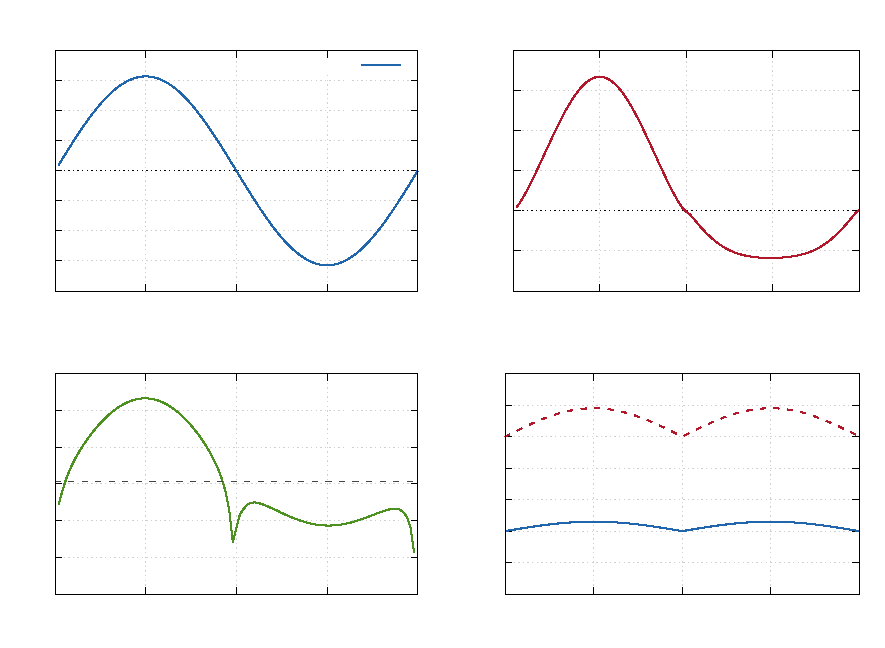
\includegraphics[width={425.00bp},height={311.00bp}]{assignment6_cycle_response}}%
    \gplfronttext
  \end{picture}%
\endgroup
